\chapter{语音信号数字处理}
\label{chap:speech_processing}

\chapternote{语音信号数字处理}{Winter 2020}

\begin{learningobjectives}
	\item 绪论
	\item 语音学基础
\end{learningobjectives}

\dependencies{无}

\section{绪论}

声波的物理描述:
\begin{enumerate}
	\item 音高 Pitch/音调: 由频率决定,单位:赫兹Hz。
	\item 音色 Timbre: 由声源本身的材料结构确定,说到底就是各个频率分量的振幅(能量)不同。
	\item 音强 Loudness/响度: 由声音增幅及离声源的距离决定,单位:分贝dB。
\end{enumerate}

\section{语音学基础}

语音产生:
\begin{enumerate}
	\item 声道
	\item 发音器官:肺,声带,软腭,阴腭,舌,牙齿,唇
	
\end{enumerate}

声带(声门)$\Rightarrow$音高$\Rightarrow$基频(源)。

\sidenotedcmmc{人的有些发音的时候声带是不震动的(清音,voiceless)。}

声道(鼻腔,口腔,鼻腔,舌头,etc)$\Rightarrow$共振特性$\Rightarrow$音色/内容(调制,\concept{滤波器})。

肺部压缩空气力量的大小$\Rightarrow$响度。

\begin{figure}[!h]
	\centerline{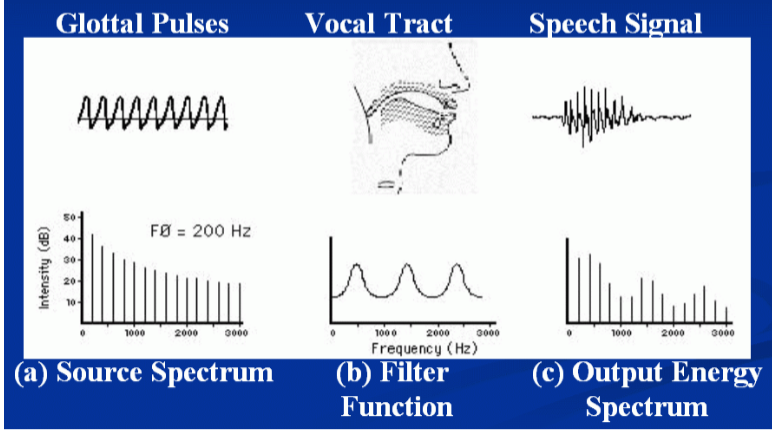
\includegraphics[width=8.0cm]{figs/speech_source_filter_model.png}}
	\caption{Source Filter Model.}
	\label{fig:Source_Filter_Model}
\end{figure}

\concept{Source-Filter Model}:

Source Spectrum(谐波)$\Rightarrow$Filter Function(每个峰值代表一个共振频率,提高/降低不同频率的增幅,不会改变频率成分) $\Rightarrow$Output Energy Spectrum.

\sidenotedcmmc{谐波就是不同频率的波叠加在一起,随着各个谐波分量频率的增加,其分量的分贝值也在下降。}

浊音 Voiced Speech:

由声带震动引起,语音波形(声门波,EGG Signal)具有明显的周期性。声带振动的频率称为基频($F_0$),人们可感受到稳定的音高存在。\emph{基频就是谐波分量中频率最低/周期最长的分量的频率}。

清音 Voiceless/Unvoiced Speech:

声带不振动,波形类似白噪声,人们无法感受到稳定的音高存在。

All languages use pitch to express emotionaland other paralinguisticinformation(超语言学信息), and to convey emphasis, contrast, and other such features in what is called intonation(语调)。

Phoneme 音位/音素:发音时不可分割的、最小的音位学单位,国际音标中每一个音标就是一个音位。

Morpheme 语素:最小的、具有语义的结构单元,是最小的语法单位,是最小的语音语义结合体。例如英语的 un-break-able,或者中文中的词语。这是 NLP 的东西,不是语音学的重点。

Viseme 视位/视素:
A visemeis a representational unit used to classify speech sounds in the visual domain, corresponding to the phoneme in the aural domain.
其实就是嘴型这种。

Bimodal Processing 双模态处理:

声音最好同时结合听觉和视觉,因为有时候同一个发音,在只听声音,只看唇形和两者结合随着三种情况下在人的感知里是三种声音(MkGurkEffect)。

Spectrum 语谱:

The spectrum of a signal is a representation of each of its frequency components and their amplitudes(振幅).

Spectrogram 语谱图:

A spectrogram is a way of envisioning how the different frequencies that make up a waveform change over time.

Wide-band Spectrogram 宽带语谱图:

频率分辨率取300-400Hz,时间分辨率2-5ms,良好的时间分辨率,频率分辨率较差。

Narrow-band Spectrogram 窄带语谱图:

频率分辨率取50-100Hz,时间分辨率5-10ms,良好的频率分辨率,时间分辨率较差。

共振峰:

是指在声音的频谱中能量相对集中的一些区域(语谱峰值)。
声音在经过共振腔时,受到腔体的滤波作用,使得频域中不同频率的能量重新分配。

\emph{第一和第二共振峰($F_1$和$F_2$) 对于区分不同元音尤为重要。}

\section{音频数字化}

\begin{enumerate}
	\item 抽样: 采样频率(抽样周期)
	\item 量化: 将无穷多个电压幅度用有限个数字表示电压幅度范围。
	\item 编码: 压缩存储
\end{enumerate}

周期信号采样后经 FFT 变换(又叫频率响应特性)为离散信号,非周期信号采样后经 FFT 变换为周期信号.
非周期信号可以复制变为周期信号, 这样就可以的到离散的频率响应特征, 离散的频率响应特征方便计算机处理和存储。

Nyquist 抽样定理:

要从抽样信号无失真地恢复信号,采样频率必须大于等于两倍信号谱的最高频率。

而以前的电话语音的采样率只有 $8k$ Hz, 这是因为该音频基本只保留谐波分量中的 $F_0, F_1, F_2$ 共振峰。
